\documentclass[addpoints]{exam}
\usepackage[utf8]{inputenc}
\usepackage[spanish]{babel}
\usepackage[T1]{fontenc}
\usepackage{charter}
\usepackage{amsmath}
\usepackage{amsfonts}
\usepackage{amssymb}
\usepackage{graphicx}
\usepackage{tikz}
\usetikzlibrary{babel,calc,patterns,decorations.pathmorphing,decorations.markings,arrows.meta,shapes.geometric}
\usepackage{tikz-3dplot}
\usepackage{multicol}
\usepackage{exam-randomizechoices}
\usepackage[left=1cm,right=1cm,top=2cm,bottom=2cm]{geometry}
\usepackage[font=small,labelfont={small,bf},margin=0.5cm,justification=justified]{caption}
\usepackage[font=small,labelfont={small,bf}]{subcaption}
\usepackage[italic,defaultmathsizes]{mathastext}
\usepackage{hyperref}
\usepackage{calculator}
\usepackage[breakable]{tcolorbox}
\usepackage{multirow}
\usepackage{tabularx}
\usepackage{cancel}
\usepackage{tipa}
\usepackage{enumerate}

%\pointpoints{punto}{puntos}
%\bonuspointpoints{punto extra}{puntos extra}

\renewcommand{\solutiontitle}{\textbf{Solución: }}
\renewcommand{\thequestion}{\bfseries\arabic{question}}

\newcommand{\sgn}{\mathop{\mathrm{sgn}}}
\newcommand{\diff}[0]{\mathrm{d}}
\newcommand{\fdiff}[2]{\frac{\mathrm{d} #1}{\mathrm{d} #2}}
\newcommand{\pdiff}[2]{\frac{\partial #1}{\partial #2}}
\newcommand{\fddiff}[2]{\frac{\mathrm{d^2} #1}{\mathrm{d} #2^2}}
\newcommand{\grado}[0]{^{\circ}}
\newcommand{\angulo}[3]{#1\grado \, #2' \, #3''}
\newcommand{\chel}[4]{^{#1}_{#2}\mbox{#3}^{#4}}
\newcommand{\valmed}[1]{\left\langle #1 \right\rangle}
\newcommand{\E}[1]{\times 10^{#1}}
\newcommand{\ver}[1]{\hat{\mathbf{#1}}}
\newcommand{\vecg}[1]{\boldsymbol{#1}}
\newcommand{\iu}{\mathrm{i}}
\newcommand{\norm}[1]{\left\vert\left\vert #1 \right\vert\right\vert}
\newcommand{\abs}[1]{\left\vert #1 \right\vert}
\newcommand{\tens}[1]{\mathbb{#1}}
\newcommand{\rr}{\mathbb{R}}
\newcommand{\un}[1]{\text{#1}}
\newcommand{\logoUNAHUR}{
\includegraphics[scale=0.35]{/home/shluna/Proyectos/Clases_Fisica_III/imgs/logo_unahur.png}}
\renewcommand{\arraystretch}{1.5}
\newcommand{\rta}{\textbf{Respuesta: }}
\newcommand{\rtas}{\textbf{Respuestas: }}
\newcommand{\ang}{110}
\newcommand{\angu}{-30}
\newcommand{\rad}{4}
\newcommand{\mg}{1}
\newcommand{\muc}{0.5}
\newcommand{\tita}{60}
\newcommand{\arc}[1]{{%
  \setbox9=\hbox{#1}%
  \ooalign{\resizebox{\wd9}{\height}{\texttoptiebar{\phantom{A}}}\cr#1}}}

\hypersetup{
%      draft,
   linktocpage=true,
    colorlinks=true,
    linkcolor=blue,
    citecolor=blue,
    filecolor=blue,      
    urlcolor=blue
}

\printanswers
\qformat{\textbf{Ejercicio \thequestion}\hfill}

\pagestyle{headandfoot}
\firstpageheader{Instituto de Tecnología e Ingeniería}{\logoUNAHUR}{Física}
\firstpageheadrule
\runningheader{Guía de ejercicios -- Unidad 1}{\logoUNAHUR}{Física}
\runningheadrule
\firstpagefooter{}{Página \thepage\ de \numpages}{}
\firstpagefootrule
\runningfooter{}{Página \thepage\ de \numpages}{}
\runningfootrule

\begin{document}

\renewcommand{\tablename}{Tabla}

\tdplotsetmaincoords{70}{110}

\begin{tcolorbox}[colback=white,arc=0mm,colframe=black]
    \begin{center}
        \Large\textbf{Guía de ejercicios resueltos y propuestos -- Unidad 1}
    \end{center}
\end{tcolorbox}

\vspace{11pt}

\begin{questions}

    \section{Tiro oblicuo}

    \question Un hombre está parado en la azotea de un edificio de $30$ m y lanza una roca con una velocidad de $40 \, \frac{\text{m}}{\text{s}}$, a $37\grado$ sobre la horizontal. Puede ignorarse la resistencia del aire. Calcule: 
    \begin{enumerate}[a)]
        \item la posición de la roca (coordenadas $x$ e $y$) a los $1$ s; $3$ s y a los $8$ s después de haber partido;
        \item la altura máxima que alcanza la roca sobre la azotea;
        \item la rapidez de la roca justo antes de golpear el suelo;
        \item la distancia horizontal desde el edificio hasta el punto donde la roca golpea el suelo;
        \item el instante en que vuelve a pasar por el nivel de la azotea.
    \end{enumerate}

    \rtas
    \begin{enumerate}[a)]
        \item $\vec{r} (1 \, \text{s}) = \left(31.95 \, \text{m} ; 49.17 \, \text{m} \right) $; $\vec{r} (3 \, \text{s}) = \left( 95.84 \, \text{m} ; 58.12 \, \text{m} \right) $; $\vec{r} (8 \, \text{s}) = \left( 255.56 \, \text{m} ; -91.02 \, \text{m} \right) $
        \item $29.38$ m;
        \item $v_\text{f} = 46.7 \, \frac{\text{m}}{\text{s}}$
        \item $d = 189.4$ m;
        \item $t = 4.91$ s.
    \end{enumerate}

    \question Se lanza una piedra horizontalmente con una velocidad inicial de 10 m/s desde un balcón de $4$ m de altura con respecto al piso. Simultáneamente, se suelta una segunda piedra del mismo punto. ¿Cuál de las dos llega primero al piso? 
    
    \rta Llegan al mismo tiempo.

    \question Un jugador de rugby patea la pelota que parte desde el piso con una velocidad de $18 \, \frac{\text{m}}{\text{s}}$ y un ángulo de $37\grado$ con respecto a la horizontal. A 30 metros de donde parte la pelota, medidos en forma horizontal, se encuentra la ``hache'' con un travesaño a 3 m de altura del piso (ver Figura~\ref{fig:rugby}). 
    \begin{enumerate}[a)]
        \item Determinar si la pelota pasa por encima o por debajo del travesaño y a qué distancia de éste lo hace.
        \item ¿En qué punto de la trayectoria la velocidad de la pelota forma un ángulo de $-30\grado$ hacia abajo con la horizontal?
    \end{enumerate}

    \begin{figure}[ht]
        \centering
        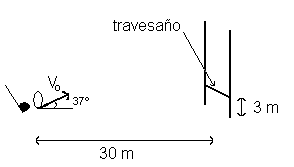
\includegraphics[scale=0.8]{/home/shluna/Proyectos/Clases_Fisica_III/figs/rugby.png}
        \caption{ }
        \label{fig:rugby}
    \end{figure}

    \rtas 
    \begin{enumerate}[a)]
        \item 2 m (aprox.) por debajo;
        \item $x=27.4$ m; $y = 2.4$ m.
    \end{enumerate}

    \question Una pelota lanzada a $53\grado$ sobre la horizontal golpea un edificio situado a 36 m en un punto a 3 m por sobre el punto de lanzamiento. Puede ignorarse la resistencia del aire. 
    \begin{enumerate}[a)]
        \item Calcule el módulo de la velocidad inicial de la bola.
        \item Obtenga el módulo y dirección de la velocidad de la pelota justo antes de golpear el edificio.
    \end{enumerate}

    \rtas
    \begin{enumerate}
        \item $v_0 = 20 \, \frac{\text{m}}{\text{s}}$;
        \item $v_\text{f} = 18.4 \, \frac{\text{m}}{\text{s}}$, $\theta = - 49.4\grado$.
    \end{enumerate}

    \question Una partícula $A$ se lanza con cierta velocidad inicial cuyo módulo es de $20 \, \frac{\text{m}}{\text{s}}$ y que forma un ángulo inicial $\theta_0$ con la horizontal, tal que $\tan \theta_0 = \frac{4}{3}$, desde una altura inicial de $10 \, \text{m}$, en el instante $t_0 = 0 \, \text{s}$. En ese mismo instante, una partícula $B$ parte del reposo en el punto $(x_0;0)$ y se desplaza hacia la derecha a lo largo del eje $x$ con aceleración constante. La Figura~\ref{fig:tiro_encuentro} muestra un esquema de la situación planteada. Despreciando el rozamiento con el aire, calcular: \label{ej:encuentro_oblicuo}
    \begin{enumerate}[a)]
        \item El instante de tiempo en el cual la partícula $A$ alcanza la altura máxima y las coordenadas de este punto, $(x_{y_\text{max}}; y_\text{max})$.
        \item El instante de tiempo ($t_{x_\text{max}})$ y las coordenadas del punto $(x_\text{max};0)$ en el que la partícula $A$ intersecta el eje $x$.
        \item El valor de la aceleración para el cual las partículas se encuentran en el instante en el que la rapidez de la partícula $B$ es igual a la componente $x$ de la velocidad de la partícula $A$.
        \item El valor de $x_0$.
    \end{enumerate}

    \textbf{Sugerencia:} Antes de comenzar a resolver el ejercicio, tenga en cuenta las condiciones iniciales de las dos partículas, es decir, en $t_0 = 0$ s:
    \begin{itemize}
        \item Partícula $A$: $x_A (0) = 0$, $y_A (0) = 10 \, \text{m}$, $v_{A,x} (0) = v_0 \cos \theta_0$, $v_{A,y} (0) = v_0 \sen \theta_0$.
        \item Partícula $B$: $x_B (0) = x_0$, $v_{B} (0) = 0$.
    \end{itemize} Escriba a continuación las ecuaciones que dan la posición y velocidad de cada partícula en función del tiempo: $x_A (t)$, $y_A (t)$, $v_{A,x} (t)$, $v_{y,A} (t)$, $x_B (t)$ y $v_B (t)$:
    \begin{table}[ht]
        \centering
        \begin{tabular}{m{0.4\textwidth}m{0.4\textwidth}}
            Partícula $A$: & Partícula $B$: \\
            $x_A (t) = $ & $x_B (t) = $ \\
            $y_A (t) = $ &  \\
            $v_{A,x} (t) = $ & $v_{B,x} (t) = $ \\
            $v_{A,y} (t) = $ & \\ 
        \end{tabular}
    \end{table} 

    Además, pensando en la condición de encuentro, responda las siguientes preguntas:
    \begin{itemize}
        \item ¿en qué punto del plano se encuentran ambas partículas?
        \item ¿cuál es el instante ($t_e$) en el que se encuentran? 
    \end{itemize}

    \question Un bloque se encuentra en el punto más alto de un plano inclinado un cierto ángulo $\theta$ respecto a la horizontal. Dicho ángulo es tal que $\tan \theta = \frac{3}{4}$. El coeficiente de rozamiento entre este y la superficie del plano es $0.25$. El bloque parte del reposo y se desplaza $10$ m hasta que llega al final del plano y cae una altura $h = 50$ m alcanzando una distancia horizontal $d$ desde el borde del plano inclinado, tal como se muestra en la Figura~\ref{fig:planoinc}. Hallar: \label{ej:planoinc_oblicuo}
    \begin{parts}
        \part La aceleración del bloque mientras se desplaza por el plano inclinado.
        \part El módulo de la velocidad del bloque cuando este llega al final del plano inclinado.
        \part El tiempo necesario para llegar al final del plano inclinado.
        \part La distancia horizontal $d$.
    \end{parts}
    
    \begin{figure}[ht]
        \centering
        \begin{subfigure}{0.5\textwidth}
            \centering
            \begin{tikzpicture}[scale=0.9]
                \draw[thick,-latex] (-0.5,0) -- (10,0) node[anchor=north]{$x$};
                \draw[thick,-latex] (0,-0.5) -- (0,5) node[anchor=east]{$y$};
                \draw[scale=1,domain=0:9,smooth,variable=\x,black,thick] plot ({\x},{-4*(\x+1)*(\x-9)/25});
                \draw[thick,-latex,red] (0,{36/25}) -- node[anchor=south east]{$\vec{v}_0$} ({2*25/sqrt(1649)},{36/25+2*32/sqrt(1649)});
                \draw (0.5,{36/25}) node[anchor=south west]{$\theta_0$} arc (0:52:0.5);
                \draw (0,{36/25}) -- (1,{36/25});
                \fill (0,{36/25}) circle (0.5mm) node[anchor=east]{$y_0$};
                \fill (4,4) circle (0.5mm);
                \draw[dashed] (0,4) -- (4,4);
                \fill (0,4) circle (0.5mm) node[anchor=east]{$y_\text{max}$};
                \draw[dashed] (4,0) -- (4,4);
                \fill (4,0) circle (0.5mm) node[anchor=north]{$x_{y_\text{max}}$};
                \fill (9,0) circle (0.5mm) node[anchor=north]{$x_\text{max}$};
                \fill (2,0) circle (0.5mm) node[anchor=north]{$x_0$};
                \draw[thick,-latex] (2,0.5) -- node[anchor=south]{$\vec{a}$} (3,0.5);
                \fill (0,0) circle (0.5mm) node[anchor=north east]{$O$};
                \node[anchor=south east] at (2,0) {$B$};
                \node[anchor=north west] at (0,{36/25}) {$A$};
            \end{tikzpicture}
            \caption{Esquema del Ejercicio~\ref{ej:encuentro_oblicuo}.}
            \label{fig:tiro_encuentro}
        \end{subfigure}
        ~
        \begin{subfigure}{0.35\textwidth}
            \centering
            \begin{tikzpicture}[scale=1.2]
                \draw[thick] (0,0) -- ({\rad*cos(\angu)},{\rad*sin(\angu)}) -- ({\rad*cos(\angu)},-5) -- ({\rad*cos(\angu)+2},-5);
                \draw ({\rad*cos(\angu)},{\rad*sin(\angu)}) -- ({\rad*cos(\angu)-1},{\rad*sin(\angu)});
                \draw ({\rad*cos(\angu)-0.5},{\rad*sin(\angu)}) arc (180.0:{180.0+\angu}:0.5);
                \node[anchor=south east] at ({\rad*cos(\angu)-0.5},{\rad*sin(\angu)}) {$\theta$};
                %%%
                \begin{scope}[rotate=\angu]
                    \draw[latex-latex] (0.3,0.75) -- node[fill=white]{$\Delta x$} (4,0.75);
                    \draw (4,0.65) -- (4,0.85);
                    \draw (0.3,0.65) -- (0.3,0.85);
                    \draw[dashed] (0.6,0.25) -- (4,0.25);
                    \draw[-latex,thick] (4,0.25) -- (5,0.25) node[anchor=west]{$\vec{v}$};
                    \draw[fill=gray!30,thick] (0,0) rectangle +(0.6,0.5);
                    %\fill (4,0.25) circle (0.5mm);
                \end{scope}
                %%%
                \fill ({4*cos(\angu)-0.25*sin(\angu)},{4*sin(\angu)+0.25*cos(\angu)}) circle (0.3mm);
                \draw ({4*cos(\angu)-0.25*sin(\angu)},{4*sin(\angu)+0.25*cos(\angu)}) -- ({4*cos(\angu)-0.25*sin(\angu)+0.75},{4*sin(\angu)+0.25*cos(\angu)});
                \draw ({4*cos(\angu)-0.25*sin(\angu)+0.5},{4*sin(\angu)+0.25*cos(\angu)}) arc (0:\angu:0.5);
                \node[anchor=north west] at ({4*cos(\angu)-0.25*sin(\angu)+0.5},{4*sin(\angu)+0.25*cos(\angu)}) {$\theta$};
                \draw[scale=1,domain={4*cos(\angu)-0.25*sin(\angu)}:{4*cos(\angu)-0.25*sin(\angu)+1.35},smooth,variable=\x,black,dashed] plot ({\x},{4*sin(\angu)+0.25*cos(\angu) + tan(\angu)*(\x-(4*cos(\angu)-0.25*sin(\angu))) - ((\x - (4*cos(\angu)-0.25*sin(\angu)))/cos(\angu))^2});
                \fill ({4*cos(\angu)-0.25*sin(\angu)+1.35},-5) circle (0.3mm);
                \draw[latex-latex] ({\rad*cos(\angu)-0.25},{\rad*sin(\angu)}) -- node[fill=white]{$h$} ({\rad*cos(\angu)-0.25},-5);
                \draw ({\rad*cos(\angu)-0.1},-5) -- ({\rad*cos(\angu)-0.4},-5);
                \draw ({\rad*cos(\angu)},-5.1) -- ({\rad*cos(\angu)},-5.4);
                \draw ({4*cos(\angu)-0.25*sin(\angu)+1.35},-5.1) -- ({4*cos(\angu)-0.25*sin(\angu)+1.35},-5.4);
                \draw[latex-latex] ({\rad*cos(\angu)},-5.25) -- node[fill=white]{$d$} ({4*cos(\angu)-0.25*sin(\angu)+1.35},-5.25);
            \end{tikzpicture}
        \caption{Esquema del Ejercicio~\ref{ej:planoinc_oblicuo}.}
        \label{fig:planoinc}
        \end{subfigure}        
    \end{figure}

    \section{Movimiento circular uniforme}

    \question ¿Qué ángulo en radianes corresponde a un arco de 90 cm de longitud situado sobre una circunferencia cuyo radio es de 60 cm? ¿Cuál es el valor de este ángulo en grados?

    \begin{solution} 
    La relación entre el ángulo en radianes ($\theta$), la longitud de arco ($s$) y el radio ($R$) de una circunferencia es: $$s = R \, \theta$$ Por lo tanto, el ángulo en radianes puede calcularse como: $$\theta = \frac{s}{R} = \frac{90 \, \text{cm}}{60 \, \text{cm}} = 1.5 \, \text{rad}$$ Para convertir esta medida a grados, podemos usar el hecho de que $360\grado = 2 \, \pi \, \text{rad}$: $$\theta = 1.5 \, \text{rad} \left(\frac{360 \grado}{2 \, \pi \, \text{rad}}\right) = \angulo{85}{56}{37.21}$$
    \end{solution}

    \question ¿Qué ángulo en radianes corresponde a un arco de 78.54 cm de longitud situado sobre una circunferencia cuyo diámetro es de 100 cm? ¿Cuál es el valor de este ángulo en grados?

    \rta $\theta = 1.5748 \, \text{rad} = \angulo{90}{13}{45.82}$.

    \question El ángulo comprendido entre dos radios de una circunferencia es $0.60$ rad. ¿Cuál es la longitud del arco correspondiente en una circunferencia de radio 200 cm?

    \rta $s = 120 \, \text{cm} = 1.20 \, \text{m}$.

    \question La tierra da una vuelta sobre sí misma una vez cada 24 hs.
    \begin{parts}
    \part Calcular la velocidad angular de rotación de la Tierra en radianes por segundo.
    \part ¿Cuántos grados se desplaza cada una hora?
    \part ¿Cuál es el módulo de la velocidad tangencial de un cuerpo situado en la superficie del ecuador terrestre?
    \end{parts}

    \begin{solution}
    \begin{parts}
        \part La Tierra da una vuelta cada 24 hs, esto significa que gira un ángulo $2 \, \pi$ radianes en 24 hs. Como sabemos que cada hora tiene 3600 segundos, entonces: $$24 \, \text{h} \left(\frac{3600 \, \text{s}}{1 \, \text{h}}\right) = 86\, 400 \, \text{s}$$ Luego: $$\omega = \frac{\Delta \theta}{\Delta t} = \frac{2 \, \pi \, \text{rad}}{86400 \, \text{s}} = \frac{\pi}{43200} \, \frac{\text{rad}}{\text{s}} \approx 7.27 \E{-5} \, \frac{\text{rad}}{\text{s}}$$
        \part El desplazamiento angular se puede calcular mediante: $$\Delta \theta = \omega \, \Delta t$$ En este caso, $\Delta t = 1 \, \text{h} = 3600 \, \text{s}$. En consecuencia: $$\Delta \theta = \frac{\pi}{43200} \, \frac{\text{rad}}{\text{s}} \times 3600 \, \text{s} = \frac{\pi}{12} \, \text{rad} \times \left(\frac{360\grado}{2 \, \pi \, \text{rad}}\right) = 15\grado$$
        \part El módulo de la velocidad tangencial viene dado por: $$ v = R_\oplus \, \omega $$ donde $R_\oplus$ es el radio de la Tierra. Teniendo en cuenta el valor antes calculado de $\omega$ y que $R_\oplus = 6.37 \E{6} \, \text{m}$, obtenemos: $$ v = 6.37 \E{6} \, \text{m} \times 7.27 \E{-5} \, \frac{\text{rad}}{\text{s}} \approx 463.01 \frac{\text{m}}{\text{s}} \approx 1667.16 \frac{\text{km}}{\text{h}}$$
    \end{parts}
    \end{solution}

    \question Calcular la velocidad angular, en radianes por segundo, del cigüeñal de un auto cuyo motor gira a 3600 rpm.

    \rta $\omega = 120 \, \pi \, \dfrac{\text{rad}}{\text{s}}$.

    \question Un motor de avión, con su hélice, se coloca sobre un banco de pruebas. Las palas de la hélice tienen, cada una, $1.8$ m de longitud.
    \begin{parts}
    \part Calcular la velocidad de los extremos de las palas cuando la hélice gira a 1200 rpm.
    \part ¿Cuál es la velocidad tangencial de un punto de la pala situado a igual distancia del eje y del extremo?
    \end{parts}

    \begin{solution}
    \begin{parts}
        \part En primer lugar, la velocidad angular es: $$\omega = 1200 \, \text{rpm} = 1200 \times \frac{2 \, \pi}{60} \, \frac{\text{rad}}{\text{s}} = 40 \, \pi \, \frac{\text{rad}}{\text{s}}$$ Luego: $$v = R \, \omega = 1.8 \, \text{m} \times 40 \, \pi \, \frac{\text{rad}}{\text{s}} = 72 \, \pi \, \frac{\text{m}}{\text{s}} \approx 226 \, \frac{\text{m}}{\text{s}} = 813.6 \, \frac{\text{km}}{\text{h}}$$
        \part La velocidad tangencial en la mitad de la distancia entre el eje y el extremo de la pala es: $$v = \frac{R}{2} \, \omega = 0.9 \, \text{m} \times 40 \, \pi \, \frac{\text{rad}}{\text{s}} = 36 \, \pi \, \frac{\text{m}}{\text{s}} \approx 113 \, \frac{\text{m}}{\text{s}} = 406.8 \, \frac{\text{km}}{\text{h}}$$
    \end{parts}
    \end{solution}

    \question Un cilindro de 15 cm de diámetro gira en un torno a 750 rpm.

    \begin{parts}
    \part ¿Cuánto vale la velocidad angular en radianes por segundo?
    \part ¿Cuál es el período de rotación?
    \part ¿Cuál es la velocidad tangencial de la superficie del cilindro?
    \part ¿Cuál es el módulo de la aceleración centrípeta?
    \part La velocidad tangencial adecuada para trabajar el hierro fundido es $60 \, \frac{\text{cm}}{\text{s}}$, aproximadamente. ¿A cuántas revoluciones por minuto debe girar en un torno, una pieza de 5 cm de diámetro?
    \end{parts}

    \begin{solution}
    \begin{parts}
        \part El cilindro gira a 750 rpm. Como $$1 \, \text{rpm} = \frac{2\, \pi}{60} \frac{\un{rad}}{\un{s}}$$ tenemos: $$ \omega = 750 \, \text{rpm} \times \left(\frac{2\, \pi}{60} \frac{\un{rad}}{\un{s}}\right) = 25 \, \pi \, \frac{\text{rad}}{\text{s}}$$
        \part El período está dado por $$P = \frac{2 \, \pi}{\omega} = \frac{2 \, \pi}{25 \, \pi \, \frac{\text{rad}}{\text{s}}} = 0.08 \, \text{s}$$
        \part La velocidad tangencial está dada por $$v = R \, \omega$$ donde $R$ es el radio de la trayectoria circular y $\omega$ es la velocidad angular expresada en radianes por segundo. Sabemos que $R = 7.5$ cm. Luego: $$v = 7.5 \, \text{cm} \times 25 \, \pi \, \frac{\text{rad}}{\text{s}} = 187.5 \, \pi \, \frac{\text{cm}}{\text{s}} \approx 589 \, \frac{\text{cm}}{\text{s}} = 5.89 \, \frac{\text{m}}{\text{s}}$$
        \part El módulo de la aceleración centrípeta viene dado por: $$a_\text{c} = v \, \omega = \frac{v^2}{R}$$ Entonces: $$a_\text{c} = 187.5 \, \pi \, \frac{\text{cm}}{\text{s}} \times 25 \, \pi \, \frac{\text{rad}}{\text{s}} = 4687.5 \, \pi^2 \, \frac{\text{cm}}{\text{s}^2} = 46.875 \, \pi^2 \, \frac{\text{m}}{\text{s}^2} \approx 462.64 \, \frac{\text{m}}{\text{s}^2}$$
        \part Ahora, tenemos que $R = 2.5 \, \text{cm}$ y que $v = 60 \, \frac{\text{cm}}{\text{s}}$. Por lo tanto, podemos calcular el valor de $\omega$: $$\omega = \frac{v}{R} = \frac{60 \, \frac{\text{cm}}{\text{s}}}{2.5 \, \text{cm}} = 24 \, \frac{\text{rad}}{\text{s}}$$ Usando nuevamente el hecho de que $$1 \, \text{rpm} = \frac{2\, \pi}{60} \frac{\un{rad}}{\un{s}}$$ se obtiene: $$24 \, \frac{\text{rad}}{\text{s}} \times \left(\frac{1 \, \text{rpm}}{\frac{2\, \pi}{60} \frac{\un{rad}}{\un{s}}}\right) \approx 230 \, \text{rpm} $$
    \end{parts}
    \end{solution}

    \question Un motor eléctrico gira a 1800 rpm y tiene sobre su eje tres poleas de diámetros 5, 10 y 15 cm, respectivamente. Calcular la velocidad tangencial en la superficie de cada polea, en metros por segundo.

    \rta Para $R = 2.5$ cm, $v = 4.71 \, \frac{\text{m}}{\text{s}}$. Para $R = 5$ cm, $v = 9.42 \, \frac{\text{m}}{\text{s}}$. Para $R = 7.5$ cm, $v = 14.14 \, \frac{\text{m}}{\text{s}}$.

    \question Hallar los valores correspondientes del módulo de la aceleración centrípeta de un punto en la superficie de cada polea. Expresarlas en metros por segundo al cuadrado.

    \rta Para $R = 2.5$ cm, $a_\text{c} = 887.36 \, \frac{\text{m}}{\text{s}^2}$. Para $R = 5$ cm, $a_\text{c} = 1774.73 \, \frac{\text{m}}{\text{s}^2}$. Para $R = 7.5$ cm, $a_\text{c} = 2665.86 \, \frac{\text{m}}{\text{s}^2}$.

    \question Una partícula, que tiene una masa de 800 g, describe una trayectoria circular de $15.7$ m de radio. El periodo de dicho movimiento es constante. Se sabe que en el instante $t_1 = 2.8$ s, la posición angular $\theta_1$ es de $15\grado$ y que en el instante $t_2 = 3.2$ s es $\theta_2 = 20\grado$. Determinar:
    \begin{parts}
    \part La frecuencia angular $\omega$.
    \part El periodo ($P$) y la frecuencia física ($f$).
    \part El módulo de la velocidad tangencial $v$.
    \part El módulo de la aceleración centrípeta $a_\text{c}$.
    \part El módulo de la fuerza centrípeta $F_\text{c}$.
    \part El momento de inercia de la partícula.
    \part El módulo del momento angular.
    \end{parts}

    \begin{solution}
    \begin{parts}
        \part Como se sabe, en $t_1 = 2.8$ s, $\theta_1 = 15\grado$ y en $t_2 = 3.2$ s, $\theta_2 = 20\grado$. La partícula describe un MCU, puesto que el periodo es constante, y por lo tanto la frecuencia angular puede calcularse como: $$ \omega = \frac{\Delta \theta}{\Delta t} = \frac{\theta_2 - \theta_1}{t_2 - t_1} = \frac{20\grado - 15\grado}{3.2\, \text{s} - 2.8 \, \text{s}} = \frac{5\grado}{0.4 \, \text{s}} = 12.5 \frac{{}\grado}{\text{s}} \approx 0.22 \frac{\text{rad}}{\text{s}}$$
        \part El periodo se puede calcular usando la relación $$ P = \frac{2 \, \pi \, \text{rad}}{\omega} = \frac{2 \, \pi \, \text{rad}}{0.22 \frac{\text{rad}}{\text{s}}} = 28.8 \, \text{s}.$$ Una vez determinado el periodo, la frecuencia física se puede calcular mediante: $$f = \frac{1}{P} = \frac{1}{28.8 \, \text{s}} \approx 0.035 \, \text{Hz} = 2.08 \, \text{rpm}$$
        \part El módulo de la velocidad tangencial se determina con la expresión: $$ v = R \, \omega = 15.7 \, \text{m} \times 0.22 \frac{\text{rad}}{\text{s}} \approx 3.42 \, \frac{\text{m}}{\text{s}}$$
        \part Podemos calcular el módulo de la aceleración centrípeta con: $$a_\text{c} = R \, \omega^2 = 15.7 \, \text{m} \times \left(0.22 \frac{\text{rad}}{\text{s}}\right)^2 \approx 0.75 \, \frac{\text{m}}{\text{s}^2}$$
        \part Multiplicando el módulo de la aceleración centrípeta antes calculado, podemos determinar el módulo de la fuerza centrípeta usando la segunda ley de Newton: $$F_\text{c} = m \, a_\text{c} = 0.8 \, \text{kg} \times 0.75 \, \frac{\text{rad}}{\text{s}^2} \approx 0.6 \, \text{N}$$
        \part A partir de su definición, el momento de inercia se calcula como: $$ I = m \, R^2 = 0.8 \, \text{kg} \times \left(15.7 \, \text{m}^2\right) = 197.19 \, \, \text{kg} \, \text{m}^2$$
        \part Por último, y aprovechando el resultado anterior, podemos calcular el módulo del momento angular: $$ L = I \, \omega \approx 197.19 \, \, \text{kg} \, \text{m}^2 \times 0.22 \frac{\text{rad}}{\text{s}} \approx 43 \, \text{kg} \, \frac{\text{m}^2}{\text{s}}$$
    \end{parts}
    \end{solution}

    \question Una pelota de 200 g de masa gira en un péndulo cónico con una cuerda de 50 cm de longitud que forma un ángulo de $10\grado$ con la vertical, describiendo un movimiento circular uniforme. Hallar:
    \begin{parts}
    \part La tensión de la cuerda.
    \part La velocidad tangencial de la pelota.
    \part El período con el que gira la pelota.
    \end{parts}

    \begin{solution}
    \begin{parts}
        \part Observando la Figura~\ref{fig:pendiloconico} se pueden obtener las componentes de los vectores tensión $\vec{T}$ y peso $\vec{F}_\text{g}$:
        \begin{align*}
        \vec{F}_\text{T} &= F_\text{T} \sen \varphi \, \ver{e}_r + F_\text{T} \cos \varphi \, \ver{e}_z \\
        \vec{F}_\text{g} &= - m \, g \, \ver{e}_z
        \end{align*} Estas son las únicas fuerzas que actúan sobre la pelota.
    
        Planteamos ahora las sumatorias de las componentes de las fuerzas en la dirección vertical y en la dirección radial:
        \begin{align*}
        R_z &= T \cos \theta - m \, g = 0 \\
        R_r &= T \sen \theta = m \, a_\text{c}
        \end{align*} De la sumatoria de fuerzas en el eje $y$ se obtiene: $$T = \frac{m \, g}{\cos \theta} = \frac{0.2 \, \text{kg} \times 9.8 \, \frac{\text{m}}{\text{s}^2}}{\cos 10\grado} \approx 2 \, \text{N}$$
        \part A partir de la sumatoria de fuerzas en el eje $x$ se puede obtener una expresión de la aceleración centrípeta: $$a_\text{c} = \frac{T \sen \theta}{m}$$ Reemplazando en esta última la expresión de la tensión obtenida antes: $$a_\text{c} = g \, \tan \theta$$ Por otro lado, la velocidad tangencial y la aceleración centrípeta se relacionan mediante: $$a_\text{c} = \frac{v^2}{R}$$ El radio de la trayectoria circular se puede obtener observando nuevamente la figura. Esto es, $R = L \sen \theta$ y por lo tanto: $$v^2 = a_\text{c} \, L \sen \theta = g \, L \, \tan \theta \sen \theta$$ Es decir: $$v = \sqrt{g \, L \, \tan \theta \sen \theta} = \sqrt{9.8 \, \frac{\text{m}}{s}^2 \times 0.5 \, \text{m} \times \tan 10\grado \times \sen 10\grado} \approx 0.387 \, \frac{\text{m}}{\text{s}}$$
        \part La aceleración centrípeta está relacionada con la velocidad angular mediante $$a_\text{c} = R \, \omega^2$$ De donde podemos despejar $\omega$: $$\omega = \sqrt{\frac{a_\text{c}}{R}} = \sqrt{\frac{g \tan \theta}{L \cos \theta}} = \sqrt{\frac{g}{L \cos \theta}}$$ Luego, podemos calcular el periodo con: $$P = \frac{2 \, \pi}{\omega} = 2 \, \pi \sqrt{\frac{L \cos \theta}{g}}$$ Reemplazando los valores: $$P = 2 \, \pi \sqrt{\frac{0.5 \, \text{m} \cos 10\grado}{9.8 \, \frac{\text{m}}{s}^2}} \approx 1.41 \, \text{s}$$
    \end{parts}
    \end{solution}

    \question Una piedra de masa 2 kg, unida a una cuerda de 50 cm de longitud y cuya resistencia a la rotura es de 500 N, gira en una circunferencia horizontal. ¿Qué velocidad debe llevar la piedra para que su velocidad angular sea la suficiente para provocar la rotura de la cuerda?

    \rta $v = 11.18 \, \frac{\text{m}}{\text{s}}$.

    \question Una pelota de 2.5 kg de masa gira en un péndulo cónico con una cuerda de 50 cm de longitud que forma un ángulo de $60\grado$ con la vertical, describiendo un movimiento circular uniforme contenido en  un plano horizontal (Figura~\ref{fig:pendiloconico}). Hallar: \label{ej:pendulo_conico}
    \begin{parts}
    \part La tensión de la cuerda.
    \part La velocidad tangencial de la pelota.
    \part El período con el que gira la pelota.
    \end{parts}

    \rtas
    \begin{parts}
        \part $T = 49$ N.
        \part $v = 2.71 \, \frac{\text{m}}{\text{s}}$.
        \part $P = 1$ s.
    \end{parts}

    \begin{figure}[ht]
        \centering
        \begin{subfigure}{0.45\textwidth}
            \centering
            \begin{tikzpicture}[scale=1,tdplot_main_coords]

                \tdplotsetthetaplanecoords{\tita}
    
    
                \coordinate (O) at (0,0,0);
    
                \draw[thick,-latex,orange,tdplot_rotated_coords] (O) -- (0,0,4) node[anchor=west]{$\theta$};
                \draw[thick,-latex,orange,tdplot_rotated_coords] (O) -- (0,0,1) node[anchor=south]{$\ver{e}_\theta$};
    
                \draw[thick,-latex,tdplot_rotated_coords,green!40!black] (0,3,0) -- (0,3,3) node[anchor=west]{$\vec{v}$};
    
                \draw[dashed] ({3*cos(\tita)},{3*sin(\tita)},0) arc (\tita:360:3);
    
                \draw[thick,-latex] (O) -- (0,4,0) node[anchor=north west]{$y$};
                \draw[ultra thick,-latex] (O) -- (0,1,0) node[anchor=west,fill=white]{$\ver{e}_y$};
    
                \fill[gray!30,tdplot_rotated_coords,opacity=0.5] (-2.3,0,0) -- (-2.3,4,0) -- (5,4,0) -- (5,0,0) -- cycle;
    
                \draw[dashed] (3,0,0) arc (0:\tita:3);
    
                \draw[thick,-latex,orange,tdplot_rotated_coords] (O) -- (0,4,0) node[anchor=west]{$r$};
                \draw[thick,-latex,orange,tdplot_rotated_coords] (O) -- (0,1,0) node[anchor=north]{$\ver{e}_r$};
    
                \draw[thick,-latex] (O) -- (4,0,0) node[anchor=north east]{$x$};
                \draw[ultra thick,-latex] (O) -- (1.5,0,0) node[anchor=south east]{$\ver{e}_x$};
    
                \draw[thick,-latex] (O) -- (0,0,5) node[anchor=south east]{$z$};
                \draw[ultra thick,-latex] (O) -- (0,0,1) node[anchor=south east]{$\ver{e}_z$};
                
                \draw[tdplot_rotated_coords,latex-latex] (O) -- node[anchor=north east]{$R$} (0,-3,0);
                \draw[thick,tdplot_rotated_coords] (4,0,0) -- node[anchor=south west]{$L$} (0,3,0);
                \tdplotdrawarc[tdplot_main_coords]{(O)}{1}{0}{\tita}{anchor=north}{$\theta$};
                \tdplotdrawarc[tdplot_main_coords,-latex]{(O)}{5}{45}{75}{anchor=north west}{$\omega$};
            
                \fill[black] (0,0,4) circle (0.5mm);
                \draw[ultra thick,tdplot_rotated_coords,-latex,red] (0,3,0) -- (-2,3,0) node[anchor=west]{$\vec{F}_\text{g}$};
                \draw[ultra thick,tdplot_rotated_coords,-latex,blue] (0,3,0) -- node[anchor=south west]{$\vec{F}_\text{T}$} (1.2,2.1,0);
                \draw[fill=gray,tdplot_rotated_coords] (0,3,0) circle (1mm);
                
                \tdplotdrawarc[tdplot_rotated_coords]{(4,0,0)}{1}{143.13}{180.0}{anchor=north}{$\varphi$};
                
                \fill[black] (O) circle (0.5mm);
            \end{tikzpicture}
            \caption{Esquema del Ejercicio~\ref{ej:pendulo_conico}.}
        \label{fig:pendiloconico}
        \end{subfigure}
        ~
        \begin{subfigure}{0.45\textwidth}
            \centering
            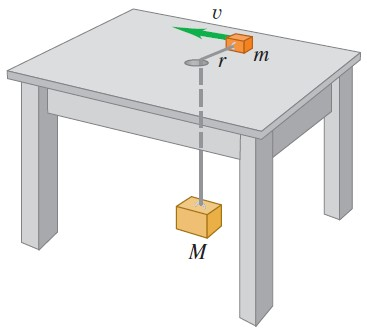
\includegraphics[width=0.6\textwidth]{/home/shluna/Proyectos/Clases_Fisica_III/figs/mesaydosmasas.jpg}
            \caption{Esquema del Ejercicio~\ref{ej:mesa}.}
            \label{fig:mesa}
        \end{subfigure}        
    \end{figure}

    \question Un bloque pequeño de masa $m$ descansa sobre una mesa horizontal sin fricción, a una distancia $r$ de un agujero en el centro de la mesa (figura~\ref{fig:mesa}). Un cordón atado al bloque pequeño pasa por el agujero y está atado por el otro extremo a un bloque suspendido de masa $M$. Se imprime al bloque pequeño un movimiento circular uniforme con radio $R$ y rapidez $v$. Obtener las expresiones de la velocidad tangencial ($v$) y del período del movimiento circular uniforme ($P$) en función de $m$, $M$ y $R$. \label{ej:mesa}

    \rta $v = \sqrt{\dfrac{M \, g \, R}{m}}$ y $P = 2 \, \pi \sqrt{\dfrac{m \, R}{M \, g}}$.

    \question Demostrar que la distancia $d$ a la cual debería colocarse un satélite artificial, de masa $m$, para que complete una trayectoria circular alrededor del centro de la Tierra en un intervalo de tiempo igual al periodo de rotación terrestre, asumiendo que este último es constante, está dada por: $$d = \sqrt[3]{\frac{G \times M_\oplus \times P^2}{4 \times \pi^2}}$$ donde $G$ es la constante gravitatoria, $M_\oplus$ es la masa de la Tierra y $P$ es el periodo del movimiento circular asociado al satélite. Una vez obtenida la expresión, calcular:
    \begin{enumerate}[a)]
        \item El valor de $d$ (expresado en metros) con los datos consignados a continuación y el valor de $\frac{d}{R_\oplus}$, donde $R_\oplus$ es el radio de la Tierra.
        \item El módulo de la velocidad tangencial, expresado en kilómetros por segundo.
    \end{enumerate}

    \textbf{Datos:} $G = 6.67 \E{-11} \dfrac{\text{N} \, \text{m}^2}{\text{kg}^2}$; $M_\oplus = 5.98 \E{24} \, \text{kg}$; $R_\oplus = 6.37 \E{6} \, \text{m}$. El periodo de rotación de la Tierra es de 86400 s.

    \begin{figure}[ht]
        \centering
        \begin{tikzpicture}[scale=1]
            \fill[gray!40] (0,0) circle (1);
            \draw[thick] (0,0) circle (1);
            \fill[black] (0,0) circle (0.5mm) node[anchor=north]{Tierra};
            \draw[thick,-latex] (0,0) -- node[anchor=north west]{$R_\oplus$} (45:1);
            \draw[thick,dashed] (0,0) circle (3);
            \draw[thick,-latex] (0,0) -- node[anchor=north east]{$d$} (120:3);
            \fill[black] (120:3) circle (0.5mm) node[anchor=south east]{Satélite};
            \node[anchor=north west] at (315:3) {Órbita del satélite};
        \end{tikzpicture}
        \caption{Esquema del ejercicio 2.}
        \label{fig:orbita_sat}
    \end{figure}

    \textbf{Sugerencia:} Asuma que la Tierra es una distribución perfectamente esférica y homogénea de masa que interactúa con el satélite a través de la fuerza de atracción gravitatoria, cuyo módulo está dado por: $$F_\text{grav} = G \, \frac{M_\oplus \, m}{d^2}$$ donde $d$ es la distancia entre el satélite artificial y el centro de la Tierra. Puede suponer, además, que la órbita del satélite está contenida en un plano que pasa por el centro de la Tierra, tal como se muestra en la Figura~\ref{fig:orbita_sat}.

    Responda las siguientes preguntas:
    \begin{itemize}
        \item ¿Cuál es el periodo del movimiento circular asociado al satélite artificial?
        \item ¿Cómo se puede calcular su frecuencia angular $\omega$?
        \item ¿Cómo están relacionadas $\omega$ y la aceleración centrípeta $a_\text{c}$?
        \item ¿Cuál es la fuerza centrípeta $F_\text{c}$ que origina la aceleración centrípeta y obliga al satélite a describir una trayectoria circular?
        \item ¿Cómo se relacionan $F_\text{c}$ y $a_\text{c}$?
    \end{itemize}

    \begin{figure}[ht]
        \centering
        \begin{tikzpicture}[scale=1,tdplot_main_coords]
            \draw[thick] (-4,-4,0) -- (4,-4,0) -- (4,4,0) -- (-4,4,0) -- cycle;
            \draw[dashed] (0,0,0) circle (3);
            \draw[fill=gray!40] (0,0,0) circle (0.1);
            \draw[fill=gray!40] ({0.1*cos(\ang)},{0.1*sin(\ang)},0) -- ({0.1*cos(\ang)},{0.1*sin(\ang)},0.5) -- ({-0.1*cos(\ang)},{-0.1*sin(\ang)},0.5) -- ({-0.1*cos(\ang)},{-0.1*sin(\ang)},0);
            \draw[fill=gray!40] (0,0,0.5) circle (0.1);
            \draw[thick] (0,-0.1,0.25) arc (-90:90:0.1);
            \draw[thick] (0,0.1,0.25) -- node[anchor=south]{$R$} (0,3,0.25);
            %\draw[thick,-Kite] (4,3,0.25) -- (3.6,3,0.25);
            %\draw[thick,red,-latex] (0,3,0.25) -- node[anchor=north west]{$\vec{v}_{\text{B}2}$} (-3,3,0.25);
            \draw[thick,-latex] (0,3,0.25) -- node[anchor=north west]{$\vec{v}_{0}$} (-3,3,0.25);
            % \draw[densely dashed] (-3,3,0.25) -- (-5,3,0.25);
            % \draw[thick,-Kite] (-5,3,0.25) -- (-5.25,3,0.25);
            % \draw[thick,-latex,blue] (-4,3.5,0.25) -- node[anchor=north west]{$\vec{v}_{\text{A}2}$} (-5.5,3.5,0.25);
            \draw[fill=gray!40] (-0.5,2.75,0) -- (-0.5,3.25,0) -- (0.5,3.25,0) -- (0.5,2.75,0) -- cycle;
            \draw[fill=gray!40] (-0.5,2.75,0.5) -- (-0.5,3.25,0.5) -- (0.5,3.25,0.5) -- (0.5,2.75,0.5) -- cycle;
            \draw[fill=gray!40] (0.5,2.75,0) -- (0.5,2.75,0.5) -- (0.5,3.25,0.5) -- (0.5,3.25,0) -- cycle;
            \draw[fill=gray!40] (0.5,3.25,0) -- (0.5,3.25,0.5) -- (-0.5,3.25,0.5) -- (-0.5,3.25,0) -- cycle;
            %\draw[densely dashed] (3.6,3,0.25) -- (0.5,3,0.25);
        \end{tikzpicture}
        \caption{ }
        \label{fig:plano_bloque_1}
    \end{figure}

    \question Un bloque de 5 kg de masa está atado a un clavo situado en el centro de una superficie horizontal sin rozamiento. Se desprecia también el efecto de cualquier otra fuerza externa, como la resistencia del aire. El hilo que une el bloque con el clavo está totalmente estirado y tiene una longitud de 25 cm. Se le imprime al bloque una velocidad inicial tal que el bloque tarda $0.1 \pi$ segundos en describir una trayectoria circular completa alrededor del clavo tal como se muestra en la Figura~\ref{fig:plano_bloque_1}. \label{ej:plano_bloque_1}

    \begin{parts}
        \part ¿Cuál es el periodo ($P$) del movimiento? Informar el valor con su respectiva unidad.
        \part Hallar la frecuencia angular ($\omega$) del movimiento.
        \part ¿Con qué rapidez describe el bloque la trayectoria circular?
        \part ¿Cuánto vale el módulo de la aceleración centrípeta?
        \part Calcular el módulo de la tensión del hilo.
    \end{parts}

    \rtas
    \begin{enumerate}[a)]
        \item $P = 0.1 \pi$ s.
        \item $\omega = 20 \, \frac{\text{rad}}{\text{s}}$.
        \item $v = 5 \, \frac{\text{m}}{\text{s}}$.
        \item $a_\text{c} = 100 \, \frac{\text{m}}{\text{s}^2}$.
        \item $F_\text{T} = 500 \, \text{N}$.
    \end{enumerate}

    \question Un proyectil que tiene una masa de 20 g se dispara contra un bloque de $4.98$ kg. El primero tiene una velocidad de $500 \, \frac{\text{m}}{\text{s}}$, mientras que el bloque está inicialmente en reposo antes de ser impactado por el proyectil. Después del choque el proyectil y el bloque quedan unidos. El bloque está atado, mediante un hilo completamente estirado de $50$ cm de longitud, a un clavo situado en el centro de una superficie sin rozamiento sobre la cual el conjunto formado por el proyectil y el bloque describe una trayectoria circular alrededor de dicho clavo, tal como se muestra en la Figura~\ref{fig:plano_bloque_2}. Determinar: \label{ej:plano_bloque_2}
    \begin{parts}
        \part La velocidad del conjunto formado por el proyectil y el bloque después del choque.
        \part La frecuencia angular $\omega$ y el periodo del movimiento circular uniforme que describe dicho conjunto.
        \part La tensión del hilo.
    \end{parts}

    \begin{figure}[ht]
        \centering
        \begin{tikzpicture}[scale=1,tdplot_main_coords]
            \draw[thick] (-4,-4,0) -- (4,-4,0) -- (4,4,0) -- (-4,4,0) -- cycle;
            \draw[dashed] (0,0,0) circle (3);
            \draw[fill=gray!40] (0,0,0) circle (0.1);
            \draw[fill=gray!40] ({0.1*cos(\ang)},{0.1*sin(\ang)},0) -- ({0.1*cos(\ang)},{0.1*sin(\ang)},0.5) -- ({-0.1*cos(\ang)},{-0.1*sin(\ang)},0.5) -- ({-0.1*cos(\ang)},{-0.1*sin(\ang)},0);
            \draw[fill=gray!40] (0,0,0.5) circle (0.1);
            \draw[thick] (0,-0.1,0.25) arc (-90:90:0.1);
            \draw[thick] (0,0.1,0.25) -- node[anchor=south]{$R$} (0,3,0.25);
            \draw[thick,-Kite] (4,3,0.25) -- (3.6,3,0.25);
            \draw[thick,-latex] (5,3.5,0.25) node[anchor=north west]{$\vec{v}_{\text{A}1}$} -- (3.5,3.5,0.25);
            %\draw[thick,red,-latex] (0,3,0.25) -- node[anchor=north west]{$\vec{v}_{\text{B}2}$} (-3,3,0.25);
            \draw[thick,-latex] (0,3,0.25) -- node[anchor=north west]{$\vec{v}_{2}$} (-3,3,0.25);
            % \draw[densely dashed] (-3,3,0.25) -- (-5,3,0.25);
            % \draw[thick,-Kite] (-5,3,0.25) -- (-5.25,3,0.25);
            % \draw[thick,-latex,blue] (-4,3.5,0.25) -- node[anchor=north west]{$\vec{v}_{\text{A}2}$} (-5.5,3.5,0.25);
            \draw[fill=gray!40] (-0.5,2.75,0) -- (-0.5,3.25,0) -- (0.5,3.25,0) -- (0.5,2.75,0) -- cycle;
            \draw[fill=gray!40] (-0.5,2.75,0.5) -- (-0.5,3.25,0.5) -- (0.5,3.25,0.5) -- (0.5,2.75,0.5) -- cycle;
            \draw[fill=gray!40] (0.5,2.75,0) -- (0.5,2.75,0.5) -- (0.5,3.25,0.5) -- (0.5,3.25,0) -- cycle;
            \draw[fill=gray!40] (0.5,3.25,0) -- (0.5,3.25,0.5) -- (-0.5,3.25,0.5) -- (-0.5,3.25,0) -- cycle;
            \draw[densely dashed] (3.6,3,0.25) -- (0.5,3,0.25);
        \end{tikzpicture}
        \caption{ }
        \label{fig:plano_bloque_2}
    \end{figure}

    \rtas
    \begin{parts}
        \part $v_2 = 2 \, \frac{\text{m}}{\text{s}}$.
        \part $\omega = 4 \, \frac{\text{rad}}{\text{s}}$; $P = 1.57 \, \text{s}$.
        \part $T = 40 \, \text{N}$.
    \end{parts}

    \pagebreak

    \section{Oscilador armónico simple}

    \question Una masa de 5 kg se sujeta a un resorte de constante $k = 500 \, \frac{\text{N}}{\text{m}}$ que se encuentra en posición horizontal (Figura~\ref{fig:oas_reposo}). Luego manualmente se estira 5 cm el resorte, tal como se muestra en la Figura~\ref{fig:oas_inicial} y se lo suelta. 
    \begin{enumerate}[a)]
        \item Hallar la frecuencia angular ($\omega$).
        \item Escribir las expresiones de $x(t)$ y de $v(t)$.
        \item Calcule la frecuencia ($f$) y el período ($P$).
        \item ¿Cuál es la rapidez máxima del cuerpo?
        \item ¿Cuándo alcanza el cuerpo por primera vez su posición de equilibrio? Calcule la aceleración en ese instante.
    \end{enumerate}

    \begin{figure}[ht]
    \centering
    \begin{subfigure}{0.45\textwidth}
        \centering
        \begin{tikzpicture}[scale=1.5]
            \draw[decoration={coil,segment length = 1mm,amplitude = 2mm,aspect = 0.3,post length = 1mm,pre length = 1mm},decorate,thick,black!50] (1,0) -- (2,0);
            \draw[thick] (1,-0.25) -- (1,0.25);
            \node at (1.5,0.3) {\scriptsize $k$};
            \draw[-latex] (0.5,0) -- (3.5,0) node[anchor=north]{\scriptsize $x$};
            \draw[-latex] (2,-0.5) -- (2,0.5) node[anchor=east]{\scriptsize $y$};
            \fill[black] (2,0) circle (0.5mm) node[anchor=south west]{\scriptsize $m$};
        \end{tikzpicture}
        \caption{ }
        \label{fig:oas_reposo}
    \end{subfigure}
    \begin{subfigure}{0.45\textwidth}
        \centering
        \begin{tikzpicture}[scale=1.5]
            \draw[decoration={coil,segment length = 2mm,amplitude = 2mm,aspect = 0.5,post length = 1mm,pre length = 1mm},decorate,thick,black!50] (1,0) -- (3,0);
            \draw[thick] (1,-0.25) -- (1,0.25);
            \draw[-latex] (0.5,0) -- (3.5,0) node[anchor=north]{\scriptsize $x$};
            \draw[-latex] (2,-0.5) -- (2,0.5) node[anchor=east]{\scriptsize $y$};
            \fill[black] (3,0) circle (0.5mm) node[anchor=south west]{\scriptsize $m$};
            \node[anchor=north] at (3,0) {\scriptsize $x_0$};
        \end{tikzpicture}
        \caption{ }
        \label{fig:oas_inicial}
    \end{subfigure}
    \caption{ }
    \label{fig:OAS}
    \end{figure}

    \begin{solution}
    \begin{enumerate}[a)]
        \item La frecuencia angular está dada por la expresión: $$\omega = \sqrt{\frac{k}{m}}$$ Teniendo en cuenta los valores correspondientes, se obtiene: $$\omega = \sqrt{\frac{500 \, \frac{\text{N}}{\text{m}}}{5 \, \text{kg}}} = \sqrt{100 \, \frac{1}{\text{s}^2}} = 10 \, \frac{\text{rad}}{\text{s}}$$
        \item La forma general de la elongación en función del tiempo es: $$x(t) = A \, \cos \left(\omega \, t + \theta_0\right),$$ donde $A$ es la amplitud del movimiento y $\theta_0$ es la fase inicial. Por otro lado, la rapidez del oscilador viene dada por: $$v(t) = - A \, \omega \sen \left(\omega \, t + \theta_0\right)$$ Si se asume que el movimiento comienza en $t= 0$, instante en el que la posición inicial del oscilador es $x_0 = 0.05 \, \text{m}$ y su rapidez inicial es nula, tenemos que: $$x(0) = A \cos \theta_0 = x_0 \qquad \text{y que} \qquad v(0) = - A \omega \sen \theta_0 = v_0$$ Podemos ver entonces que, en términos generales: $$A = \sqrt{x_0^2 + \left(\frac{v_0}{\omega}\right)^2} \qquad \text{y} \qquad \tan \theta_0 = - \frac{v_0}{\omega \, x_0}$$ Como $v_0 = 0$, entonces $$A = \sqrt{x_0^2} = \abs{x_0} = 0.05 \, \text{m}$$ y $$\tan \theta_0 = - \frac{0}{\omega \, x_0} = 0$$ El hecho de que $\tan \theta_0 = 0$ podría significar, en principio que $\theta_0 = 0$ o que $\theta_0 = \pi$, pero como $x_0 > 0$, entonces es evidente que la solución correspondiente es $\theta_0 = 0$. Así, las expresiones de la elongación y de la rapidez en función del tiempo son 
        \begin{align*}
        x(t) &= 0.05 \, \text{m} \cos \left(10 \, \frac{\text{rad}}{\text{s}} \, t\right); \\
        v(t) &= - 0.05 \, \text{m} \times 10 \, \frac{\text{rad}}{\text{s}} \sen \left(10 \, \frac{\text{rad}}{\text{s}} \, t\right) = - 0.5 \, \frac{\text{m}}{\text{s}} \sen \left(10 \, \frac{\text{rad}}{\text{s}} \, t\right)
        \end{align*}
        \item La frecuencia ``física'' $f$ está relacionada con la frecuencia angular mediante: $$\omega = 2 \, \pi \, f$$ Entonces: $$f = \frac{\omega}{2 \, \pi} = \frac{10 \, \frac{\text{rad}}{\text{s}}}{2 \, \pi} = \frac{5}{\pi} \frac{1}{\text{s}} \approx 1.59 \, \text{Hz}$$ Por otra parte, el periodo se puede calcular usando la expresión $$P = \frac{2 \, \pi}{\omega}$$ o bien: $$P = \frac{1}{f}$$ De cualquiera de las dos formas se obtiene: $$P = \frac{\pi}{5} \, \text{s} \approx 0.63 \, \text{s}$$
        \item La rapidez máxima del oscilador puede pensarse como la ``amplitud'' de la función periódica $v(t)$, es decir: $$v_\text{max} = 0.5 \, \frac{\text{m}}{\text{s}}$$
        \item El instante en que el oscilador alcanza por primera vez la posición de equilibrio se puede determinar de la siguiente manera. En virtud de que $$\omega = \frac{2 \, \pi}{P}$$ podemos reescribir, de forma general, la expresión de $x(t)$ como: $$ x(t) = A \cos \left(\frac{2 \, \pi}{P} \, t\right)$$ Se llamamos $t_\text{eq}$ a dicho instante, entonces: $x(t_\text{eq}) = 0$, entonces: $$x(t_\text{eq}) = A \cos \left(\frac{2 \, \pi}{P} \, t_\text{eq}\right) = 0$$ Esto es: $$\cos \left(\frac{2 \, \pi}{P} \, t_\text{eq}\right) = 0$$ Como sabemos, el coseno es cero ``por primera vez'' cuando su argumento es igual a $\frac{\pi}{2}$, luego: $$\frac{2 \, \pi}{P} \, t_\text{eq} = \frac{\pi}{2},$$ de donde se obtiene que $$t_\text{eq} = \frac{P}{4}$$ Así, podemos observar que el oscilador alcanza la posición de equilibrio por primera vez después de que ha transcurrido un intervalo de tiempo igual a la cuarta parte del periodo del mismo. Entonces: $$t_\text{eq} \approx 0.158 \, \text{s}$$ Por último, en el instante en que el oscilador pasa por la posición de equilibrio, en virtud de la relación $a(t) = - \omega^2 x(t)$, resulta claro que la aceleración debe ser igual a cero en dicho instante.
    \end{enumerate}
    \end{solution}

    \question Un proyectil, que tiene $20 \, \un{g}$ de masa y se desplaza a una velocidad de $200 \, \frac{\text{m}}{\text{s}}$ en dirección horizontal y sentido hacia la derecha, choca contra un bloque de masa $1.98 \, \un{kg}$ que se encuentra en reposo sobre una superficie horizontal lisa, y queda incrustado en él. El bloque esta unido a un resorte en hélice como indica la Figura~\ref{fig:bala_bloque_resorte}. El calibrado del resorte indica que para comprimirlo $1 \, \un{cm}$ es necesaria una fuerza de $2 \, \un{N}$. Luego del choque, el sistema formado por el proyectil, el bloque y el resorte, describe un movimiento armónico simple.
        
    Determinar:
    \begin{parts}
    \part La velocidad del conjunto formado por el bloque y el proyectil inmediatamente después del choque.
    \part La frecuencia angular ($\omega$) y el periodo ($P$) del oscilador armónico simple.
    \part Las ecuaciones que dan la posición, la velocidad y la aceleración del oscilador en función del tiempo en la forma: 
    \begin{itemize}
        \item $x(t) = \phantom{-} \, A \cos \left(\omega \, t + \theta_0\right)$.
        \item $v(t) = - \, A \, \omega \sen \left(\omega \, t + \theta_0\right)$.
        \item $a(t) = - \, A \, \omega^2 \cos \left(\omega \, t + \theta_0\right)$.
    \end{itemize}
    \part ¿Cuál es el valor máximo del módulo de la aceleración?
    \end{parts}

    \begin{figure}[ht]
        \centering
        \begin{subfigure}{0.45\textwidth}
            \centering
            \begin{tikzpicture}[scale=1]
                \draw[decoration={coil,segment length = 3mm,amplitude = 2mm,aspect = 0.75,post length = 1mm,pre length = 1mm},decorate,thick,black!50] (2,0.5) -- (5,0.5);
                \draw[fill=gray!40] (1,0) rectangle (2,1);
                \node at (1.5,0.5) {$m$};
                \node at (3.5,1) {$k$};
                \draw[thick] (0,0) -- (5,0) -- (5,1);
                
                \coordinate (A) at (0,0.5);  % To position the bullet in another fig
                \begin{scope}[shift={(A)}, rotate=0,scale=0.1]
                \fill[top color=black!10, bottom color=black!70]
                (0,1) -- (1.5, 1) to [out=0, in=120] (2.5,0.5) to[out=-120, in=0] (1.5,0) -- (0,0) --cycle;
                \draw[white, draw opacity=0.5, line cap=round, line width=0.8mm] (0,0.1) -- (1.5,0.1) to[out=0, in=-140] (2.5,0.5)  (0.02,0) -- (0.02,1) (0.2,0) -- (0.2,1);
                \draw[black!80, line width=0.4mm]   (0,1) -- (1.5, 1) to [out=0, in=120] (2.5,0.5) to[out=-120, in=0] (1.5,0) -- (0,0) --cycle (0.18,0) -- (0.18,1);
                \end{scope}
                \draw[thick,-latex] (-0.25,1) -- node[anchor=south]{$\vec{v}$} (0.5,1);
            \end{tikzpicture}
            \caption{}
            \label{fig:bala_bloque_resorte1}
        \end{subfigure}
        ~
        \begin{subfigure}{0.45\textwidth}
            \centering
            \begin{tikzpicture}[scale=1]
                \draw[decoration={coil,segment length = 2mm,amplitude = 2mm,aspect = 0.5,post length = 1mm,pre length = 1mm},decorate,thick,black!50] (3.5,0.5) -- (5,0.5);
                \draw[fill=gray!40] (2.5,0) rectangle (3.5,1);
                \draw (1,1.1) -- (1,1.4);
                \draw (2.5,1.1) -- (2.5,1.4);
                \draw [latex-latex] (1,1.25) -- node[fill=white]{$\Delta L$} (2.5,1.25);
                \draw[thick] (0,0) -- (5,0) -- (5,1);
                \coordinate (A) at (2.5,0.5);  % To position the bullet in another fig
                \begin{scope}[shift={(A)}, rotate=0,scale=0.1]
                \fill[top color=black!10, bottom color=black!70]
                (0,1) -- (1.5, 1) to [out=0, in=120] (2.5,0.5) to[out=-120, in=0] (1.5,0) -- (0,0) --cycle;
                \draw[white, draw opacity=0.5, line cap=round, line width=0.8mm] (0,0.1) -- (1.5,0.1) to[out=0, in=-140] (2.5,0.5)  (0.02,0) -- (0.02,1) (0.2,0) -- (0.2,1);
                \draw[black!80, line width=0.4mm]   (0,1) -- (1.5, 1) to [out=0, in=120] (2.5,0.5) to[out=-120, in=0] (1.5,0) -- (0,0) --cycle (0.18,0) -- (0.18,1);
                \end{scope}
            \end{tikzpicture}
            \caption{}
            \label{fig:bala_bloque_resorte2}
        \end{subfigure}
        \caption{ }
        \label{fig:bala_bloque_resorte}
    \end{figure}

    \begin{solution}
    \begin{enumerate}[a)]
        \item La velocidad del conjunto formado por el proyectil y el bloque después del choque puede hallarse utilizando la ecuación: $$m_A \, v_{A1} + m_B \, v_{B1} = m_A \, v_{A2} + m_B \, v_{B2},$$ donde $m_A$ y $m_B$ son la masa del proyectil y la del bloque, respectivamente, $v_{A1}$ y $v_{A2}$ son la rapidez del proyectil antes y después del choque, respectivamente, y $v_{B1}$ y $v_{B2}$ son las correspondientes para el bloque. En virtud de que el bloque estaba en reposo antes del choque, tenemos que $v_{B1} = 0$. Además, como ambos quedan unidos después del choque, sus velocidades son iguales: $v_{A2} = v_{B2} = v_2$. Entonces: $$m_A \, v_{A1} = \left(m_A + m_B\right) v_2$$ de donde podemos determinar el valor de $v_2$: $$v_2 = \frac{m_A \, v_{A1}}{m_A + m_B}$$ Reemplazando los valores correspondientes: $$v_2 = \frac{0.02 \, \text{kg} \times 200 \, \frac{\text{m}}{\text{s}}}{0.02 \, \text{kg} + 1.98 \, \text{kg}} = 2 \, \frac{\text{m}}{\text{s}}$$
        \item Como sabemos, tanto la frecuencia angular como el periodo del oscilador armónico simple depende únicamente de $k$ y de $m$, mediante: $$ \omega = \sqrt{\frac{k}{m}} \qquad \text{ y } \qquad P = \frac{2\, \pi}{\omega} = 2 \, \pi \sqrt{\frac{m}{k}}$$ En este caso, tenemos que el resorte se comprime un centímetro cada 2 N de fuerza que se le aplica. Por lo tanto: $$k = 2 \frac{\text{N}}{\text{cm}} = 200 \, \frac{\text{N}}{\text{m}}$$ Además, la masa del oscilador es igual a la masa del conjunto formado por el proyectil y el bloque: $m = m_A + m_B = 2 \, \text{kg}$. Luego: $$\omega = \sqrt{\frac{200 \, \frac{\text{N}}{\text{m}}}{2 \, \text{kg}}} = \sqrt{100 \, \frac{1}{\text{s}^2}} = 10 \, \frac{\text{rad}}{\text{s}}$$ Entonces, el periodo es: $$ P = \frac{2 \, \pi \,\text{rad}}{10 \, \frac{\text{rad}}{\text{s}}} = \frac{\pi}{5} \text{s} \approx 0.63 \, \text{s}$$
        \item Para poder escribir las ecuaciones que dan la elongación, la rapidez y la aceleración en función del tiempo, debemos primero determinar el valor de la amplitud y de la fase inicial. Una manera es considerando las condiciones iniciales. En $t= 0$, el oscilador se encuentra en la posición de equilibrio y su velocidad inicial es igual a $v_2$ en virtud del impulso adquirido inmediatamente después del choque. Esto es:
        \begin{align*}
        x(0) &= A \cos \theta_0 = 0 \\
        v(0) &= - \, A \, \omega \sen \theta_0 = v_2 \Rightarrow A \sen \theta_0 = - \frac{v_2}{\omega}.
        \end{align*} Por un lado, podemos elevar ambos miembros de estas dos ecuaciones y luego sumarlas para obtener: $$A = \sqrt{\left(\frac{v_2}{\omega}\right)^2} = \abs{\frac{v_2}{\omega}}$$ Reemplazando los valores correspondientes, obtenemos: $$ A = \abs{\frac{2 \, \frac{\text{m}}{\text{s}}}{10 \, \frac{\text{rad}}{\text{s}}}} = 0.2 \, \text{m}$$ Por otro lado, podemos calcular el cociente entre la segunda y la primera: $$\frac{A \sen \theta_0}{A \cos \theta_0} = \frac{- \frac{v_2}{\omega}}{0}$$ Lo que es equivalente a: $$ \tan \theta_0 = \frac{- \frac{v_2}{\omega}}{0} $$ Como el numerador es negativo y el denominador es nulo, $\tan \theta_0$ tiende a $-\infty$ y, por lo tanto: $$\theta_0 = \frac{3 \, \pi}{2}$$ En consecuencia:
        \begin{align*}
        x(t) &= 0.2 \, \text{m} \cos \left(10 \, \frac{\text{rad}}{\text{s}} \, t + \frac{3 \, \pi}{2}\right) \\
        v(t) &= - 2 \, \frac{\text{m}}{\text{s}} \sen \left(10 \, \frac{\text{rad}}{\text{s}} \, t + \frac{3 \, \pi}{2}\right) \\
        a(t) &= 20 \, \frac{\text{m}}{\text{s}^2} \cos \left(10 \, \frac{\text{rad}}{\text{s}} \, t + \frac{3 \, \pi}{2}\right)
        \end{align*}
        \item El valor máximo de la aceleración corresponde a la ``amplitud'' de la función periódica que da la aceleración del oscilador en función del tiempo, es decir: $$a_\text{max} = 20 \, \frac{\text{m}}{\text{s}^2}$$
    \end{enumerate}
    \end{solution}

    \question Un oscilador armónico está formado por una masa de 100 kg y un resorte de constante $k$ desconocida.
    \begin{parts}
        \part Si el período de las oscilaciones es $P=1$ s, determinar la constante elástica $k$.
        \part Si el resorte se reemplaza por otro de $k = 156.8 \, \frac{\text{N}}{\text{m}}$ y la masa por otra de valor $m = 10$ kg, hallar la frecuencia de las oscilaciones.
    \end{parts}

    \rtas
    \begin{parts}
        \part $k = 3950 \frac{\text{N}}{\text{m}}$.
        \part $f = 0.63$ Hz.
    \end{parts}

    \question Un cuerpo de masa 10 g se mueve con movimiento armónico simple, de amplitud 24 cm y $P = 4$ s. Cuando $t=0$, la elongación es de $+24$ cm. Calcular:
    \begin{parts}
        \part La posición del cuerpo en $t=0.5$ s.
        \part El valor y el sentido de la fuerza que actúa sobre el cuerpo en $t=0.5$ s.
        \part El tiempo mínimo que es necesario para que se mueva desde la posición inicial hasta el punto de elongación $x = -12$ cm.
        \part La velocidad del cuerpo para $x=-12$ cm.
    \end{parts}

    \rtas
    \begin{parts}
        \part $x = 17$ cm.
        \part $F = -0.42 \E{-2}$ N.
        \part $t = 1.33$ s.
        \part $v = \pm 32.6 \, \frac{\text{cm}}{\text{s}}$.
    \end{parts}

    \question Hallar el periodo de oscilación de una partícula, sabiendo que cuando la elongación es de $6.25$ cm la aceleración es de $1 \, \frac{\text{m}}{\text{s}^2}$.

    \rta $P = 1.57$ s.

    \question Un cuerpo de masa 300 kg oscila en el extremo de un resorte sobre una superficie horizontal sin rozamiento. En el gráfico de la Figura~\ref{fig:graficaOAS} se observa la posición del cuerpo en función del tiempo.
    \begin{parts}
        \part Calcule la constante elástica del resorte.
        \part Calcule la velocidad máxima que adquiere el cuerpo.
        \part ¿En qué instantes la aceleración tiene módulo máximo?
    \end{parts}

    \begin{figure}[ht]
        \centering
        \begin{tikzpicture}[scale=1]
            \draw[-latex,thick] (-0.5,0) -- (10,0) node[anchor=north]{\scriptsize $t$ [s]};
            \draw[-latex,thick] (0,-2) -- (0,2) node[anchor=east]{\scriptsize $x(t)$ [cm]};
            \draw[scale=1,domain=0:9,smooth,variable=\x,red,thick] plot ({\x},{1.5*cos(deg(2*pi*\x/6))});
            \fill (0,1.5) circle (0.5mm) node[anchor=east]{\scriptsize $5$};
            \fill (0,-1.5) circle (0.5mm) node[anchor=east]{\scriptsize $-5$};
            \fill (0,0) circle (0.5mm) node[anchor=north east]{\scriptsize $0$};
            \fill (1.5,0) circle (0.5mm) node[anchor=north]{\scriptsize $2$};
            \fill (3,0) circle (0.5mm) node[anchor=north]{\scriptsize $4$};
            \fill (4.5,0) circle (0.5mm) node[anchor=north]{\scriptsize $6$};
            \fill (6,0) circle (0.5mm) node[anchor=north]{\scriptsize $8$};
            \fill (7.5,0) circle (0.5mm) node[anchor=north east]{\scriptsize $10$};
            \fill (9,0) circle (0.5mm) node[anchor=north]{\scriptsize $12$};
        \end{tikzpicture}
        \caption{ }
        \label{fig:graficaOAS}
    \end{figure}

    \rtas
    \begin{parts}
        \part $k=185 \, \frac{\text{N}}{\text{m}}$.
        \part $0.039 \, \frac{\text{m}}{\text{s}}$. 
        \part $0$ s, 4 s y 8 s.
    \end{parts}

    \question Un cuerpo de masa $0.25$ kg está sometido a una fuerza recuperadora elástica de constante de $25 \, \frac{\text{N}}{\text{m}}$. Se inicia la oscilación del cuerpo con una energía potencial de $0.6$ J y una energía cinética de $0.2$ J.
    \begin{parts}
        \part ¿Cuál es la amplitud de movimiento?
        \part ¿Cuál es la $E_\text{pe}$ cuando la elongación es la mitad de la amplitud?
        \part ¿Para qué elongación son iguales la $E_\text{c}$ y la $E_\text{pe}$?
        \part ¿Cuál es la velocidad del cuerpo en el centro de su trayectoria?
    \end{parts}

    \rtas
    \begin{parts}
        \part $0.25$ m.
        \part $0.2$ J.
        \part $x = \pm 0.18$ m.
        \part $v = \pm 2.59 \, \frac{\text{m}}{\text{s}}$.
    \end{parts}

    \question Para el sistema del problema anterior, hallar:
    \begin{parts}
        \part El período $P$.
        \part La frecuencia $f$.
        \part La frecuencia angular $\omega$.
        \part La fase inicial $\theta_0$ si la amplitud es $A =15$ cm, la elongación inicial es $x_0 =7.5$ cm y la velocidad inicial $v_0$ es negativa.
        \part Escribir las ecuaciones horarias del movimiento: $x(t)$, $v(t)$ y $a(t)$.
    \end{parts}

    \rtas
    \begin{parts}
        \part $P = 0.628$ s.
        \part $f = 1.59$ Hz.
        \part $\omega = 10 \, \frac{\text{rad}}{\text{s}}$.
        \part $\theta_0 = \frac{5 \, \pi}{6} \, \text{rad}$. 
    \end{parts}

    \question Un oscilador armónico simple está formado por una masa puntual de $5$ kg y un resorte cuya constante es $2880\, \frac{\text{N}}{\text{m}}$, tal como se muestra en la Figura~\ref{fig:OAS_x0neg} (\subref{fig:oas_reposo_x0neg}). El resorte se comprime hasta el punto $(-50 \, \text{cm};0)$, tal como se muestra en la Figura~\ref{fig:OAS_x0neg} (\subref{fig:oas_inicial_x0neg}) y luego el sistema se libera partiendo del reposo.

    \begin{figure}[ht]
        \centering
        \begin{subfigure}{0.45\textwidth}
            \centering
            \begin{tikzpicture}[scale=1.75]
                \draw[decoration={coil,segment length = 2mm,amplitude = 2mm,aspect = 0.5,post length = 1mm,pre length = 1mm},decorate,thick,black!50] (0,0) -- (2,0);
                \draw[thick] (0,-0.25) -- (0,0.25);
                \node at (1,0.3) {$k$};
                \draw[-latex] (-0.5,0) -- (4,0) node[anchor=north]{$x$};
                \draw[-latex] (2,-0.5) -- (2,0.5) node[anchor=east]{$y$};
                \fill[black] (2,0) circle (0.5mm) node[anchor=south west]{$m$};
            \end{tikzpicture}
            \caption{ }
            \label{fig:oas_reposo_x0neg}
        \end{subfigure}
        \begin{subfigure}{0.45\textwidth}
            \centering
            \begin{tikzpicture}[scale=1.75]
                \draw[decoration={coil,segment length = 1mm,amplitude = 2mm,aspect = 0.3,post length = 1mm,pre length = 1mm},decorate,thick,black!50] (0,0) -- (1,0);
                \draw[thick] (0,-0.25) -- (0,0.25);
                \node at (0.5,0.3) {$k$};
                \draw[-latex] (-0.5,0) -- (4,0) node[anchor=north]{$x$};
                \draw[-latex] (2,-0.5) -- (2,0.5) node[anchor=east]{$y$};
                \fill[black] (1,0) circle (0.5mm) node[anchor=south west]{$m$};
                \node[anchor=north] at (1,-0.1) {$x_0$};
            \end{tikzpicture}
            \caption{ }
            \label{fig:oas_inicial_x0neg}
        \end{subfigure}
        \caption{ }
        \label{fig:OAS_x0neg}
    \end{figure}

    \begin{parts}
        \part Determinar 
        \begin{subparts}
            \subpart la amplitud ($A$),
            \subpart la frecuencia angular ($\omega$)
            \subpart el periodo ($P$) y
            \subpart la frecuencia física ($f$).
        \end{subparts} de las oscilaciones.
        \checkboxchar{$\Box$}
        \part ¿Para qué valores de $x$ la rapidez de la masa puntual alcanza su valor máximo? Seleccionar todas las opciones correctas: \\
        \begin{oneparcheckboxes}
            \choice $-0.5$ m,
            \choice 0 m,
            \choice $0.5$ m.
        \end{oneparcheckboxes}
        \part ¿Para qué valores de $x$ la rapidez de la masa puntual se anula? Seleccionar todas las opciones correctas: \\ 
        \begin{oneparcheckboxes}
            \choice $-0.5$ m,
            \choice 0 m,
            \choice $0.5$ m.
        \end{oneparcheckboxes}
        \part ¿Para qué valores de $x$ el módulo de la aceleración impresa a la masa puntual alcanza su valor máximo? Seleccionar todas las opciones correctas: \\
        \begin{oneparcheckboxes}
            \choice $-0.5$ m,
            \choice 0 m,
            \choice $0.5$ m.
        \end{oneparcheckboxes}
        \part ¿Para qué valores de $x$ el módulo de la aceleración impresa a la masa puntual se anula? Seleccionar todas las opciones correctas: \\
        \begin{oneparcheckboxes}
            \choice $-0.5$ m,
            \choice 0 m,
            \choice $0.5$ m.
        \end{oneparcheckboxes}
        \part Si se duplica la amplitud, ¿se modifican los valores de $P$, $f$, $\omega$ y los resultados de los ítems (b), (c), (d) y (e)? ¿Por qué? Seleccione la respuesta correcta a continuación:
        \checkboxchar{$\bigcirc$}
        \begin{checkboxes}
            \choice Sí, porque al duplicarse la amplitud, se duplican tanto la velocidad como la aceleración y por lo tanto los instantes de tiempo en los que el cuerpo pase por la posición de equilibrio van a ser diferentes.
            \choice No, porque $\omega$, y por lo tanto $f$ y $P$, no dependen de las condiciones iniciales.
            \choice No es posible determinar si los resultados se modifican o no con la información disponible.
        \end{checkboxes}
    \end{parts}

    \rtas
    \begin{enumerate}[a)]
        \item
        \begin{itemize}
            \item $A =0.5$ m.
            \item $\omega =24 \, \frac{\text{rad}}{\text{s}}$.
            \item $P = 0.26$ s.
            \item $f = 3.82$ Hz.
        \end{itemize}
        \item $ x = 0$ m.
        \item $ x = -0.5$ m; $x = 0.5$ m.
        \item $ x = -0.5$ m; $x = 0.5$ m.
        \item $ x = 0$ m.
    \end{enumerate}

    \section{Dinámica rotacional y MCUV}

    \question Un péndulo está constituido por una pequeña esfera de plomo, de masa 100 g, sujeta al extremo de una cuerda de 1 m de longitud. ¿Cuál es su momento de inercia respecto a un eje que pasa por el extremo superior de la cuerda y es perpendicular a su longitud?

    \begin{solution}
        Consideremos la esfera como una masa puntual. El momento de inercia es: $$I = m \, L^2 = 0.1 \, \text{kg} \times \left(1 \, \text{m}\right)^2 = 0.1 \, \text{kg m}^2$$
    \end{solution}

    % \question Durante intervalos de 2 segundos de duración, se han realizado las lecturas en el tacómetro de un motor que se muestran en la Tabla~\ref{tab:tacometro}

    % \begin{table}[ht]
    % \centering
    % \begin{tabular}{|c|c|c|c|c|c|c|c|c|c|c|}
    %     \hline
    %     Tiempo (s)              & 0    & 2    & 4    & 6    & 8    & 10   & 12   & 14   & 16   & 18   \\ \hline
    %     Velocidad angular (rpm) & 1000 & 1000 & 1500 & 2000 & 2500 & 3000 & 3500 & 3800 & 4000 & 4000 \\ \hline
    % \end{tabular}
    % \caption{ }
    % \label{tab:tacometro}
    % \end{table}

    % Calcular la aceleración angular media, en radianes por segundo cuadrado, durante cada intervalo de dos segundos. ¿Fue constante la aceleración angular durante el intervalo total? ¿Lo fue durante alguna parte del intervalo?

    % \begin{solution}
    % En el intervalo comprendido entre 0 y 2 segundos no hubo cambio de velocidad angular, tampoco en el intervalo entre 16 y 18 segundos. Por lo tanto, durante dichos intervalos la aceleración angular fue nula. En el intervalo comprendido entre 2 y 4 segundos la velocidad angular aumentó desde 1000 a 1500 rpm, es decir, de 105 a 157 $\frac{\text{rad}}{\text{s}}$. El aumento de velocidad angular fue de, por consiguiente, $\Delta \omega = 157 \, \frac{\text{rad}}{\text{s}} - 105 \, \frac{\text{rad}}{\text{s}} = 52 \, \frac{\text{rad}}{\text{s}}$, y puesto que el intervalo de tiempo $\Delta t$ fue de 2 segundos, la aceleración  angular media fue de: $$\alpha = \frac{\Delta \omega}{\Delta t} = \frac{52 \, \frac{\text{rad}}{\text{s}}}{2 \, \text{s}} = 26 \, \frac{\text{rad}}{\text{s}^2}$$ 
    % \end{solution}

    \question Una partícula de masa $m = 1.2 \, \text{kg}$ describe una trayectoria circular de radio $R = 5 \, \text{m}$. En el instante $t_1 = 4.25 \, \text{s}$, la frecuencia angular de esta es $\omega_1 = 15 \frac{{}\grado}{\text{s}}$, mientras que en el instante $t_2 = 6.5 \, \text{s}$ su frecuencia angular es $\omega_2 = 45 \, \frac{{}\grado}{\text{s}}$. Determinar:
    \begin{parts}
    \part el valor medio de la aceleración angular media,
    \part el momento de inercia de la partícula y
    \part el valor medio de la componente del torque perpendicular al plano del movimiento.
    \end{parts}

    \begin{solution}
    \begin{parts}
        \part En virtud de los datos presentes en la consigna del ejercicio, podemos determinar la aceleración angular utilizando la expresión: $$ \valmed{\alpha} = \frac{\Delta \omega}{\Delta t} = \frac{\omega_2 - \omega_1}{t_2 - t_1}$$ Reemplazando los valores correspondientes, se obtiene: $$\valmed{\alpha} = \frac{45 \, \frac{{}\grado}{\text{s}} - 15 \frac{{}\grado}{\text{s}}}{6.5 \, \text{s} - 4.25 \, \text{s}} = \frac{30 \, \frac{{}\grado}{\text{s}}}{2.25 \, \text{s}} \approx 0.23 \frac{\text{rad}}{\text{s}^2}$$
        \part El momento de inercia de la partícula respecto del punto alrededor del cual describe la trayectoria circular es: $$ I = m \, R^2 = 1.2 \, \text{kg} \times \left(5 \, \text{m}\right)^2 = 30 \, \text{kg} \, \text{m}^2 $$
        \part Por último, el valor medio del torque es: $$ \valmed{\tau} = I \, \valmed{\alpha} = 30 \, \text{kg} \, \text{m}^2 \times 0.23 \frac{\text{rad}}{\text{s}^2} = 6.98 \, \text{N m}.$$
    \end{parts}
    \end{solution}

    \question En un determinado instante, una partícula de masa $m = 6 \, \text{kg} $ se encuentra sobre el eje $x$ de cierto sistema de referencia a $4.5 \, \text{m}$ a la derecha de su origen y sobre ella actúa una fuerza que tiene un módulo de $500 \, \text{N}$ y forma un ángulo de $30\grado$ con la parte positiva del eje $x$, tal como se muestra en la Figura~\ref{fig:torque}. Determinar el módulo del torque producido por la fuerza y el módulo de la aceleración angular, ambos medidos en el sistema de referencia dado.

    \begin{figure}[ht]
    \centering
        \begin{tikzpicture}[scale=1]
        \draw[thick,-latex] (0,-0.5) -- (0,1.5) node[anchor=east]{$y$};
        \draw[thick,-latex] (-0.5,0) -- (7,0) node[anchor=north]{$x$};
        \draw[thick,-latex,red] (4.5,0) -- node[anchor=south east]{$\vec{F}$} ({4.5+2*cos(30)},1);
        \draw (5,0) arc (0:30:0.5);
        \node[anchor=south west] at (5.1,0) {$30\grado$};
        \fill[black] (0,0) circle (0.5mm);
        \fill[black] (4.5,0) circle (0.5mm);
        \draw[latex-latex] (0,-0.3) -- node[fill=white]{$4.5 \, \text{m}$} (4.5,-0.3);
        \draw (4.5,-0.1) -- (4.5,-0.5);
        \end{tikzpicture}
    \caption{ }
    \label{fig:torque}
    \end{figure}

    \begin{solution}
    A partir de la Figura~\ref{fig:torque}, podemos ver que el vector de posición de la partícula es: $$\vec{r} = (4.5 \, \text{m} ; 0). $$ Por otro lado, las componentes de la fuerza aplicada sobre la partícula son: $$\vec{F} = \left(F \cos \theta; F \sen \theta \right),$$ donde $F = \norm{\vec{F}} = 500 \, \text{N}$ y $\theta = 30\grado$. En consecuencia, el torque es: $$ \vec{\tau} = \vec{r} \times \vec{F} = \left(500 \, \text{N} \sen 30\grado \times 4.5 \, \text{m} - 0 \times 500 \, \text{N} \cos 30\grado\right) \hat{\vec{k}} = 1125 \, \text{N m} \, \hat{\vec{k}}. $$ de donde se concluye que $\norm{\vec{\tau}} = 1125 \, \text{N m}$.

    El torque y la aceleración angular están relacionados mediante: $$ \vec{\tau} = I \, \vec{\alpha}. $$ Sin embargo, como ambos vectores son paralelos y tienen la misma dirección que el eje $z$, perpendicular al plano $x-y$, podemos trabajar directamente con sus módulos: $$ \tau = I \, \alpha, $$ donde $I = m \, R^2$ es el momento de inercia. Para este caso: $$ I = 6 \, \text{kg} \times \left(4.5 \, \text{m}\right)^2 = 121.5 \, \text{kg} \, \text{m}^2. $$ Luego: $$\alpha = \frac{\tau}{I} = \frac{1125 \, \text{N m}}{121.5 \, \text{kg} \, \text{m}^2} = 9.26 \, \frac{\text{rad}}{\text{s}^2}.$$
    \end{solution}

    \question Un disco de radio 10 cm parte del reposo y comienza a girar alrededor de un eje horizontal que pasa por su centro con una aceleración angular de $2 \, \frac{\text{rad}}{\text{s}^2}$. Calcular al cabo de 1 segundo:
    \begin{parts}
    \part la velocidad angular;
    \part el desplazamiento angular;
    \part el módulo de la aceleración centrípeta;
    \part el modulo de la aceleración tangencial;
    \part el módulo de la aceleración resultante.
    \end{parts}

    \begin{solution}
    \begin{parts}
        \part $$\omega = \omega_0 + \alpha \, \Delta t = 2 \, \frac{\text{rad}}{\text{s}^2} \times 1 \, \text{s} = 2 \, \frac{\text{rad}}{\text{s}}$$
        \part $$\Delta \theta = \omega_0 \, \Delta t + \frac{1}{2} \alpha \, \Delta^2 = \frac{1}{2} \times 2 \, \frac{\text{rad}}{\text{s}^2} \times 1^2 \, \text{s}^2 = 1 \, \text{rad}$$
        \part $$a_\text{c} = R \, \omega^2$$ $$\omega^2 = \omega_0^2 + 2 \, \alpha \, \Delta \theta = 2 \times 2 \, \frac{\text{rad}}{\text{s}^2} \, \times 1 \, \text{rad} = 4 \, \frac{\text{rad}^2}{\text{s}^2}$$ $$a_\text{c} = 10 \, \text{cm} \times 4 \, \frac{\text{rad}^2}{\text{s}^2} = 40 \, \frac{\text{cm}}{\text{s}^2}$$
        \part $$a_\text{t} = R \, \alpha = 10 \, \text{cm} \times 2 \, \frac{\text{rad}}{\text{s}^2} = 20 \, \frac{\text{cm}}{\text{s}^2}$$
        \part $$a = \sqrt{a_\text{c}^2 + a_\text{t}^2} = \sqrt{\left(40 \, \frac{\text{cm}}{\text{s}}\right)^2 + \left(20 \, \frac{\text{cm}}{\text{s}^2}\right)^2} = 45.7 \, \frac{\text{cm}}{\text{s}^2}$$
    \end{parts}
    \end{solution}

    \question Si ahora se considera que hay rozamiento entre el bloque y la superficie horizontal del Ejercicio~\ref{ej:plano_bloque_2}, siendo el coeficiente cinético de rozamiento $\mu_\text{c} = 0.1$, y se le imprime la misma velocidad inicial ($v_0 = 2 \, \frac{\text{m}}{\text{s}}$), determinar:
    \begin{parts}
        \part el valor de la componente $z$ de la aceleración angular y el de la aceleración tangencial y
        \part el intervalo de tiempo transcurrido desde que el bloque inicia su movimiento hasta que se detiene completamente y el desplazamiento angular correspondiente.
    \end{parts}

    \textbf{Dato:} El radio de la trayectoria circular es de 50 cm.

    \rtas
    \begin{parts}
        \part $\alpha = - 1.96 \, \frac{\text{rad}}{\text{s}^2}$; $ a_\text{t} = - 0.98 \, \frac{\text{m}}{\text{s}^2}$.
        \part $\Delta t = 2.04 \, \text{s}$; $\Delta \theta = 4.08 \, \text{rad}$.
    \end{parts}

    \question Se considera nuevamente la situación esquematizada en la Figura~\ref{fig:plano_bloque_1}, pero esta vez se desconoce la masa del bloque y la longitud del hilo que une al bloque con el clavo es ahora de 50 cm. Además, se considera que hay rozamiento entre el bloque y la superficie horizontal, siendo $\mu_\text{c} = 0.1$, y se le imprime al bloque una velocidad inicial tal que este logra dar una vuelta completa alrededor del clavo antes de detenerse completamente.
    \begin{parts}
        \part Calcular el valor inicial de la frecuencia angular ($\omega_0$).
        \part Hallar el valor del intervalo de tiempo ($\Delta t$) que tarda el bloque en dar la vuelta completa.
    \end{parts}

    \rtas
    \begin{enumerate}[a)]
        \item $\omega_0 = 4.96 \, \frac{\text{rad}}{\text{s}}$.
        \item $\Delta t = 2.53$ s.
    \end{enumerate}

\end{questions}

    \begin{table}[ht]
        \centering
        \begin{tabular}{|c|cccccccccc|}
            \hline
            $\alpha$ (grados)   & $0\grado$ &  $30\grado$ & $45\grado$ & $60\grado$ & $90\grado$ & $135\grado$ & $180\grado$ & $225\grado$ & $270\grado$ & $315\grado$ \\
            \hline
            $\alpha$ (radianes) &   $0$    &  $\frac{\pi}{6}$ & $\frac{\pi}{4}$ & $\frac{\pi}{3}$ & $\frac{\pi}{2}$ & $\frac{3}{4} \pi$ & $\pi$ & $\frac{5}{4} \pi$ & $\frac{3}{2} \pi$ & $\frac{7}{4} \pi$ \\
            \hline
            $\sin \alpha$       &   $0$    & $\frac{1}{2}$ & $\frac{\sqrt{2}}{2}$ & $\frac{\sqrt{3}}{2}$ & $1$ & $\frac{\sqrt{2}}{2}$ & $0$ & $\frac{-\sqrt{2}}{2}$ & $-1$ & $-\frac{\sqrt{2}}{2}$ \\
            $\cos \alpha$       &   $1$    & $\frac{\sqrt{3}}{2}$ & $\frac{\sqrt{2}}{2}$ & $\frac{1}{2}$ & $0$ & $-\frac{\sqrt{2}}{2}$ & $-1$ & $-\frac{\sqrt{2}}{2}$ & $0$ & $\frac{\sqrt{2}}{2}$ \\
            $\tan \alpha$       &   $0$    & $\frac{\sqrt{3}}{3}$ & $1$ & $\sqrt{3}$ & $+\infty$ & $-1$ & $0$ & $1$ & $-\infty$ & $-1$ \\
            \hline  
        \end{tabular}
    \end{table}

\end{document}